\documentclass{article} % For LaTeX2e
\usepackage[legalpaper, margin=0.16in]{geometry}
\usepackage{amsmath}
\usepackage{amsfonts,dsfont}
\usepackage{amssymb}
\usepackage[ruled,vlined]{algorithm2e}

\usepackage{graphicx}
\usepackage{caption}
\usepackage{subcaption}
\usepackage{xcolor}
\usepackage{siunitx}

\begin{document}

\begin{figure}
	\centering
	\captionsetup{labelformat=empty}
	\begin{subfigure}{0.30\textwidth}
		%% trim=left bottom right top
		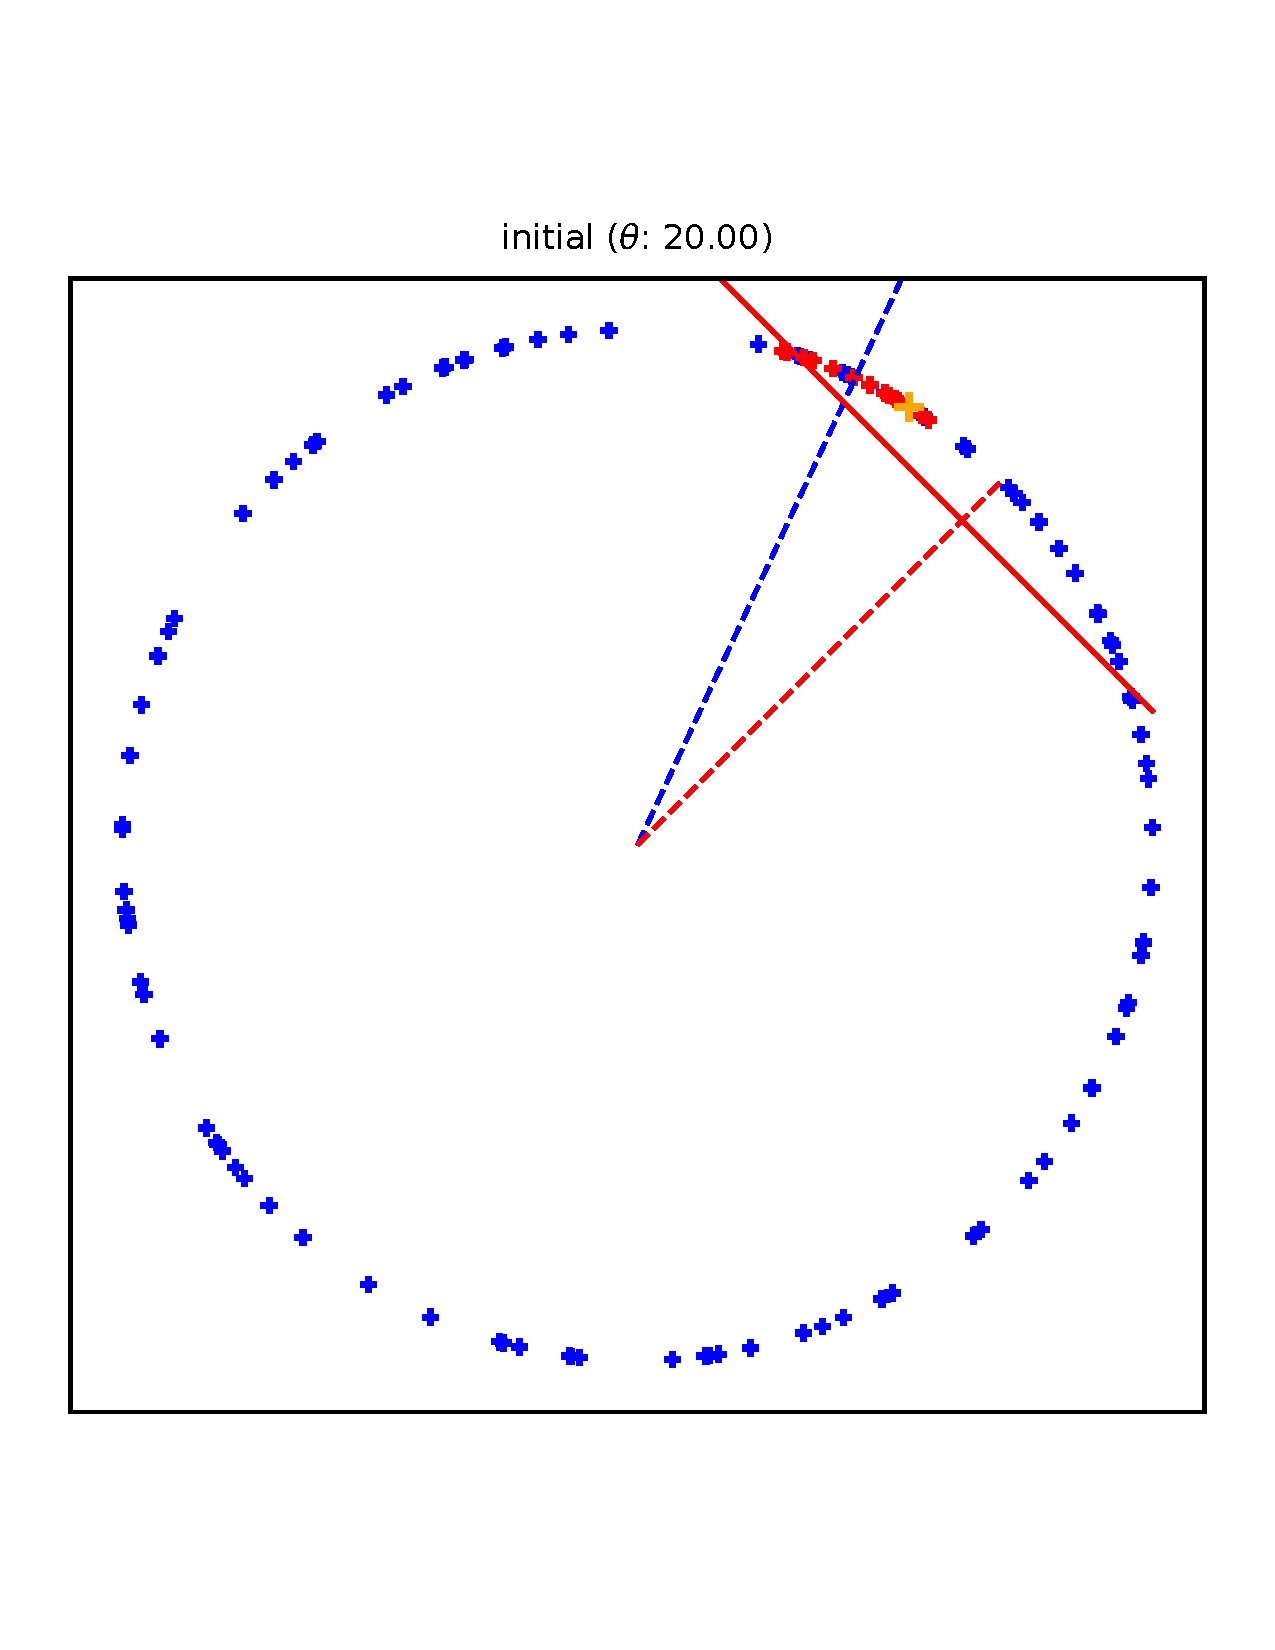
\includegraphics[width=\textwidth, clip=true, trim=12mm 40mm 12mm 35mm]{iter_00}
		\caption{Initialize weights to uniform}
		\label{fig:iter_00}
	\end{subfigure}
	\begin{subfigure}{0.30\textwidth}
		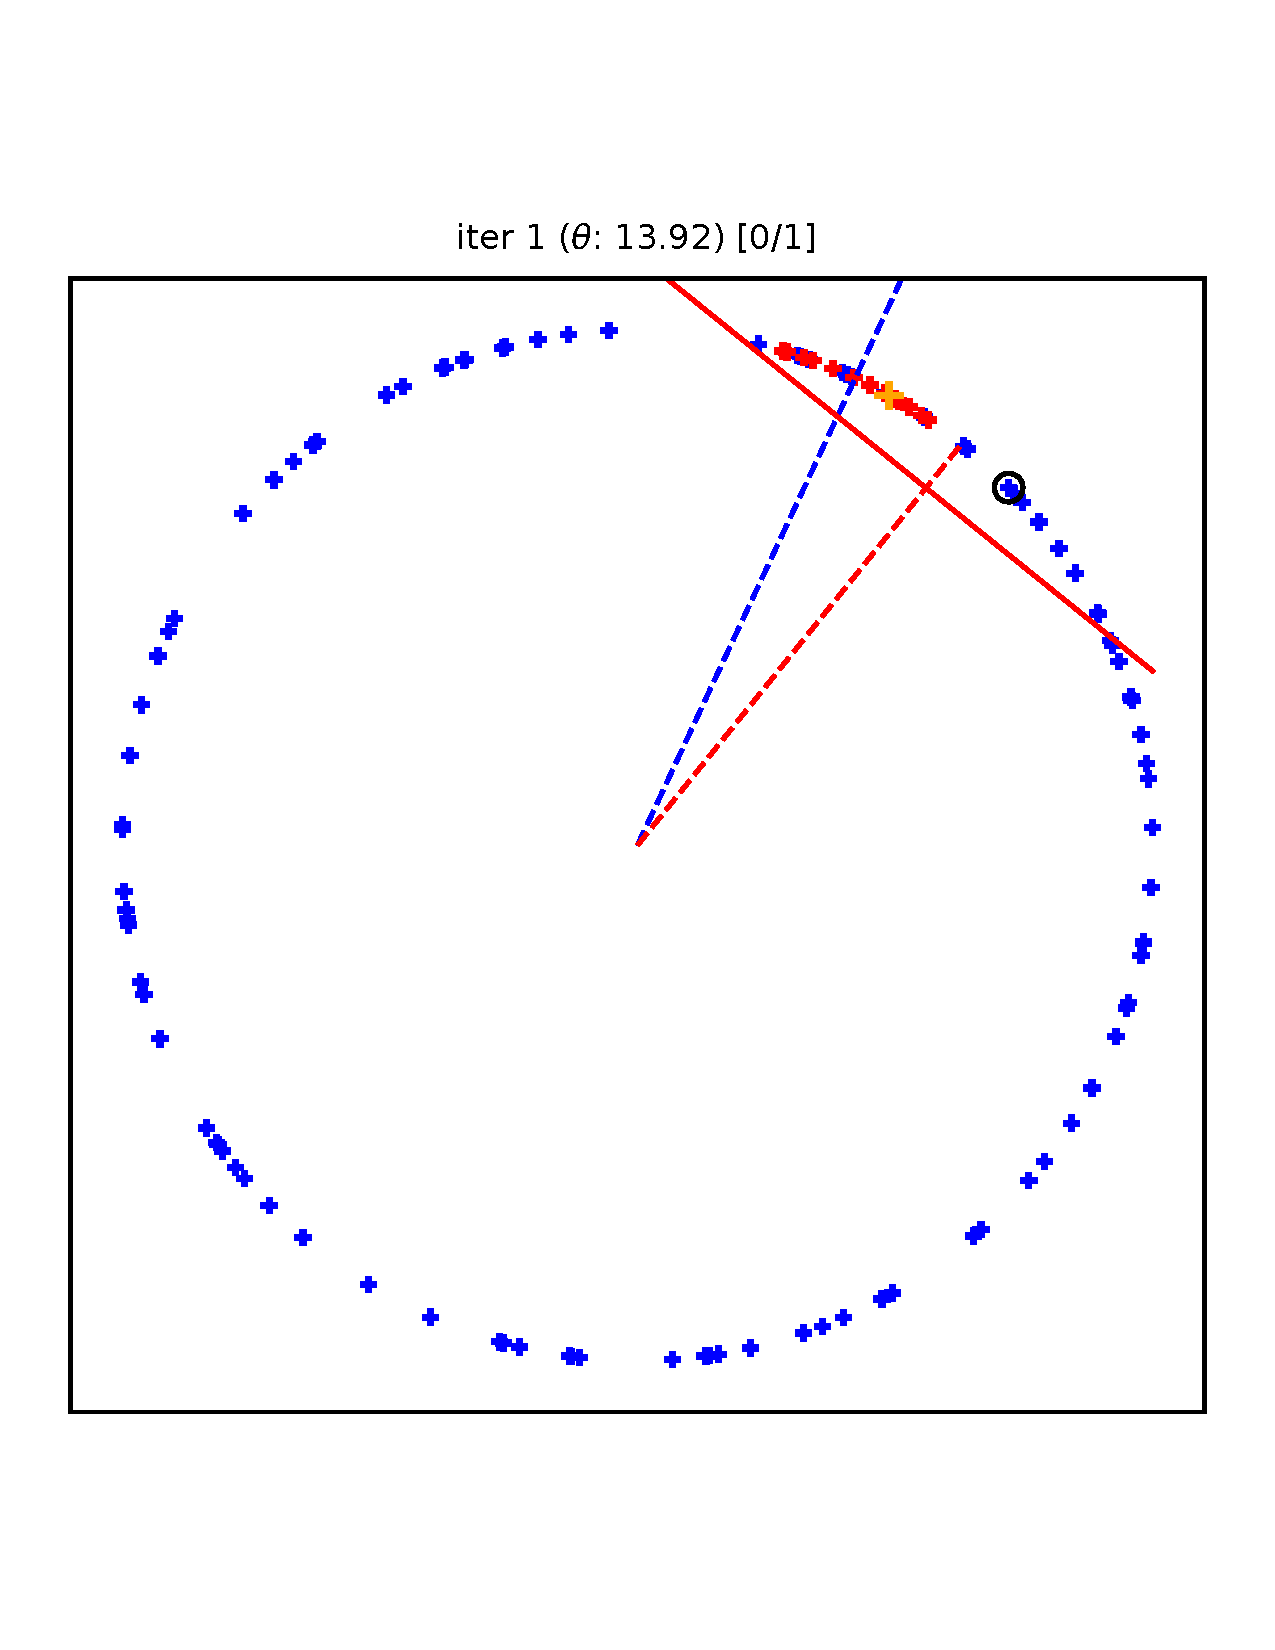
\includegraphics[width=\textwidth, clip=true, trim=12mm 40mm 12mm 35mm]{iter_01}
		\caption{After first feedback}
		\label{fig:iter_01}
	\end{subfigure}
	\begin{subfigure}{0.30\textwidth}
		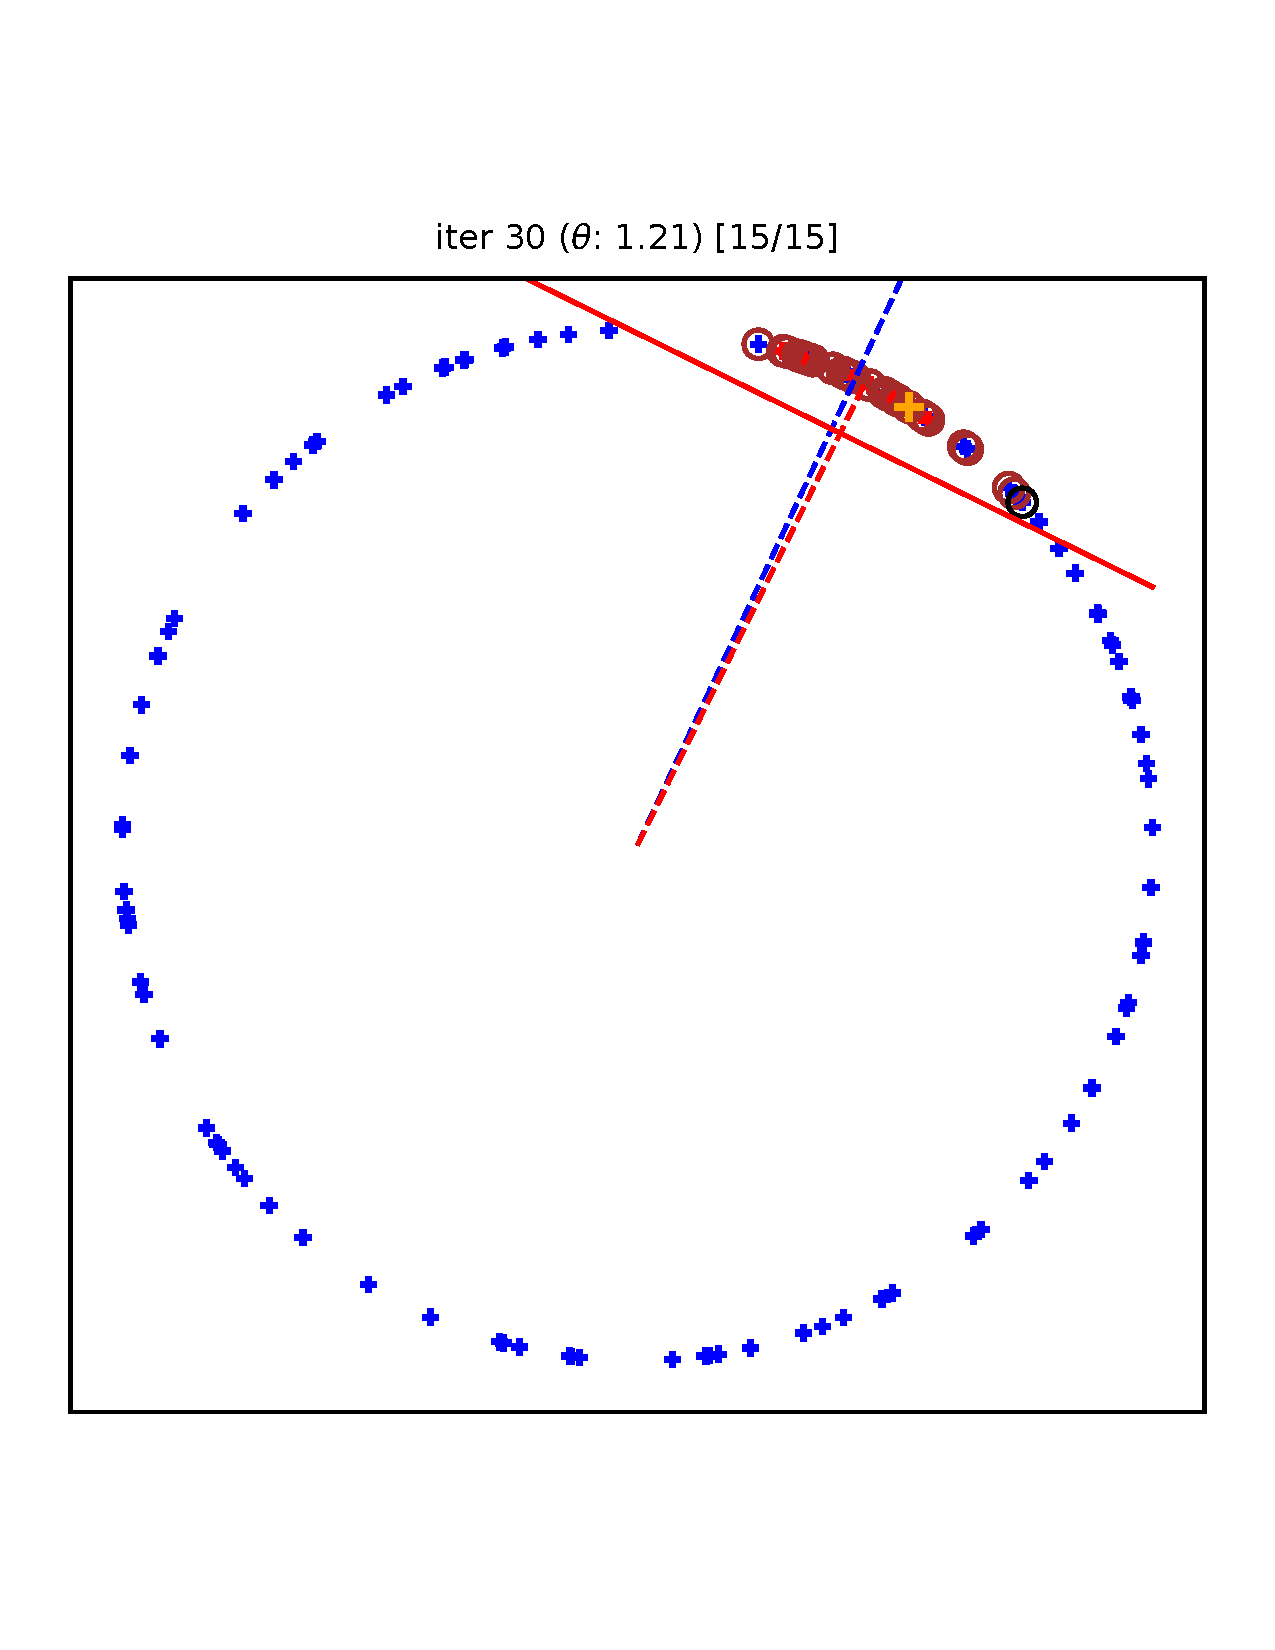
\includegraphics[width=\textwidth, clip=true, trim=12mm 40mm 12mm 35mm]{iter_30}
		\caption{After 30 feedback}
		\label{fig:iter_30}
	\end{subfigure}
	\caption{Simplified illustration of AAD. Points in \textbf{\textcolor{blue}{blue}} are nominals, and points in \textcolor{red}{red} are anomalies. The dashed-\textcolor{red}{red} line is the \textbf{current} weight vector, the solid-\textcolor{red}{red} line is the hyperplane perpendicular to the current weight vector. The dashed-\textcolor{blue}{blue} line represents the \textbf{true} weight vector that we need to \textbf{learn} through feedback. The \textbf{\textcolor{orange}{`+'}} represents the point with $\tau$-th quantile score. The \textbf{\textcolor{black}{black circle}} is the point labeled in the current iteration. The \textbf{\textcolor{brown}{brown}} circles represent all points labeled in past iterations. The uniform weight, which is our \textit{starting} point (Fig.(a)), is displaced by an angle $\theta=\ang{20}$ from the true weight vector. The very first instance ranked at the top is a nominal (Fig.(b)). The true weights have been approximately learned by $30$ iterations (Fig.(c)), and all $15$ anomalies discovered as well (in this case). Points near the hyperplane are in the \textit{uncertain} region. By making sure that only a small fraction of top-ranked instances are on one side of the margin, AAD ensures that the top-ranked instances are close to the hyperplane and therefore in the region of uncertainty. Querying these instances then allows AAD to benefit from uncertainty sampling. Anomaly detector ensembles have the property that the true hyperplane normal is close to uniform weights, which provides a good starting point for active learning.} \label{fig:percept}
\end{figure}

\end{document}
